\chapter{psi46test}

This software package is mainly targeted to chip and module testing at low levels. For more detector driven aspects consider using \texttt{psi46expert}.

\section{Basic chip test}

%=============================================
\section{Command reference}

%---------------------------------------------
\subsection{Power and chip control}
\begin{description}
    \cmditem{pon}{} %Power on

    Turns on the power currents $VD$ and $VA$ for the chip/module and activates the signals.
    \cmditem{poff}{}%Power off

    Safely turns off the power currents for the chip/module and inactivates the signals. Does not turn off the bias voltage.

\end{description}

%---------------------------------------------
\subsection{DTB information}
\begin{description}
    \cmditem{rpcinfo}{} 

    This shows a list of all RPC function the installed firmware supports. Check this for debugging purposes.
\end{description}

%---------------------------------------------
\subsection{Pattern generator}
\begin{description}
    \cmditem{rpcinfo}{step pattern delay} 

    Used to define a signal pattern to be issued once or repeatedly. A sequence consists of up to 255 \emph{step}s, enumeration starts at 0. The \emph{pattern} is a binary value to select signals. The \emph{delay} parameter defines the number of clock cycles with no activity after the pattern has been sent out. A \emph{delay} value of 0 marks the end of a sequence.
\end{description}

%---------------------------------------------
\subsection{Analog signals}
\begin{description}
    \cmditem{showclk}{} %Show a oscilloscope view of the CLK signal

    Displays the CLK signal vs. time. No adjustments can be made. Shows it in a graphics window separated from the terminal. Caution: alters settings for timing and signal routing. See Fig.~\ref{fig:DTBscopes} for an example.
    \cmditem{showctr}{}

    Displays the calibrate--trigger--reset sequence of signals vs. time. No adjustments can be made. Shows it in a graphics window separated from the terminal. Caution: alters settings for timing, signal generator and signal routing. See Fig.~\ref{fig:DTBscopes} for an example.
    \cmditem{showsda}{} %

    Displays the analog data SDATA1 showing a pixel readout. No adjustments can be made. Shows it in a graphics window separated from the terminal. Caution: alters settings for timing, signal generator and signal routing. See Fig.~\ref{fig:DTBscopes} for an example.
\end{description}

\begin{figure}[hbtp]
    \begin{center}
	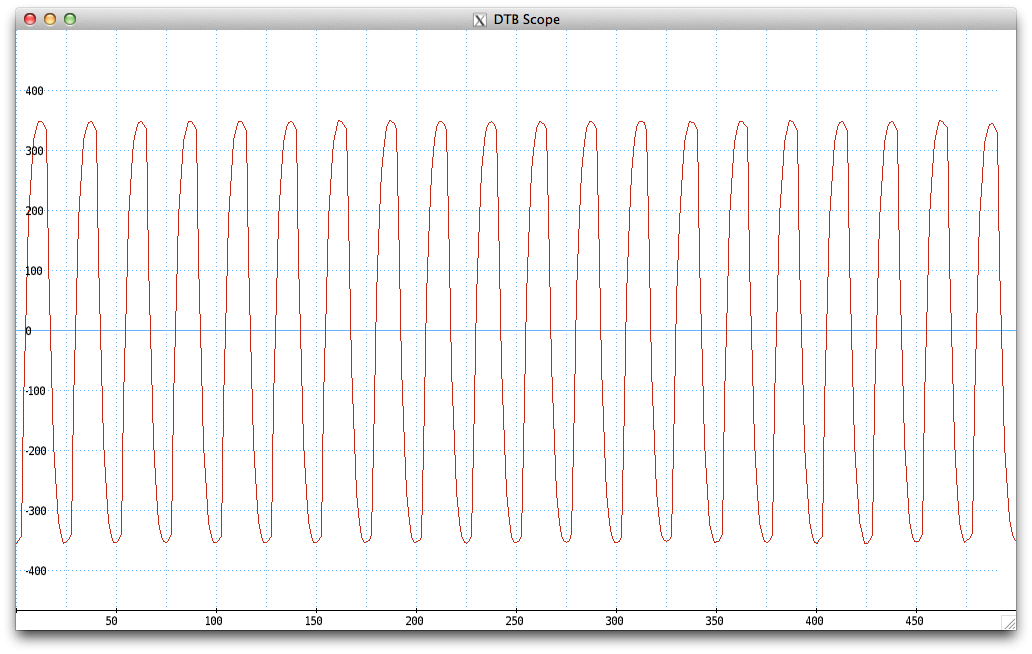
\includegraphics[width=0.70\textwidth]{img/scope_clk.png}
	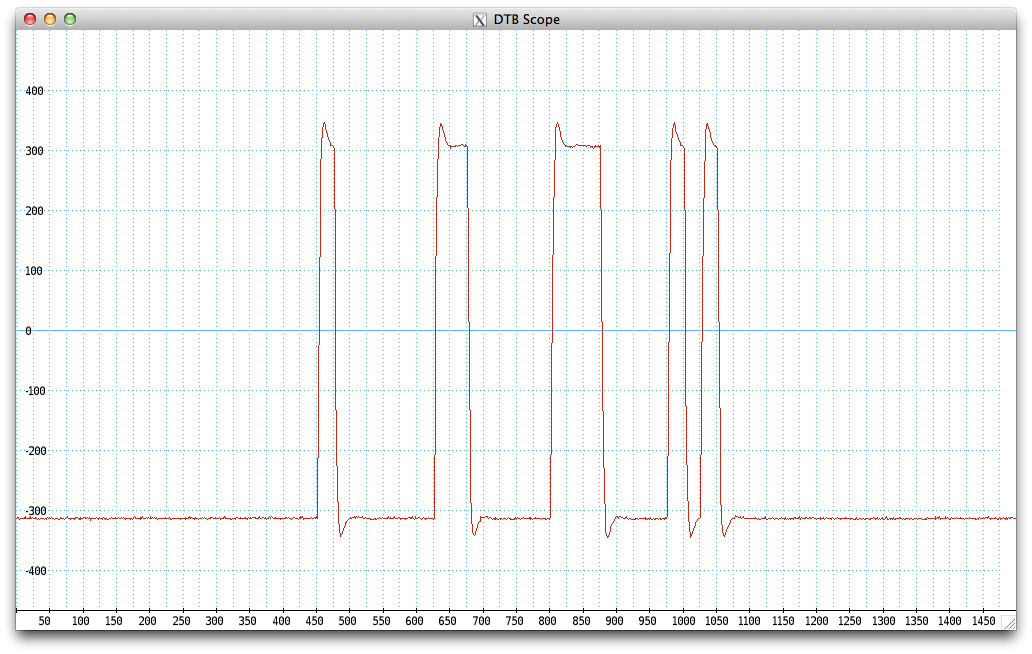
\includegraphics[width=0.70\textwidth]{img/scope_ctr.png}
	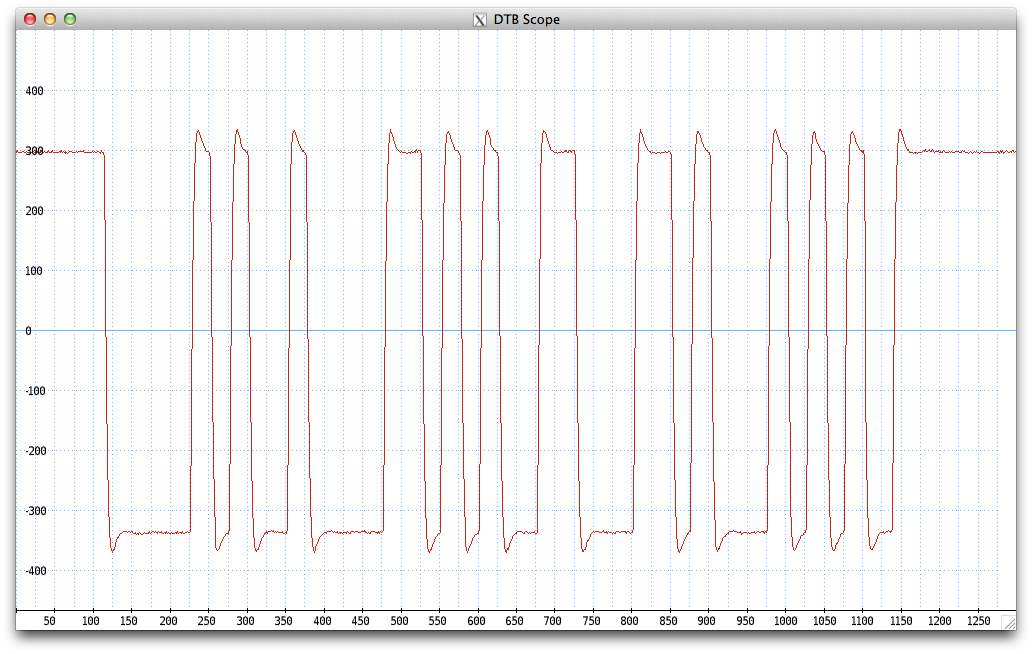
\includegraphics[width=0.70\textwidth]{img/scope_sda.png}
	\caption{Examples of plots shown by commands \texttt{showclk} (top), \texttt{showctr} (center), and \texttt{showsda} (bottom).}
	\label{fig:DTBscopes}
    \end{center}
\end{figure}

